% !TEX root = ../main.tex
\section{全向干扰源的自动搜索、定位与清除策略}

\subsection{问题分析与总体思路}

问题三要求机器狗在半径 $1800\,\mathrm m$ 的圆域内搜索并清除 $10$--$16$ 个全向干扰源。干扰源占用 $20$ 个频道中的不同频道，其位置、频道和有效接收半径均未知。机器狗从原点出发，测向机初始频道为 1；每次检测只能得到“无信号”“距离过近”或带 $\pm1^\circ$ 误差的示向度。因此，本问不仅需要延续前两问的几何定位方法，还要同时决定检测频道、检测位置和清除时机。

对照实际程序，本文采用“\textbf{保守可行域保证正确性，几何采样评分提高效率}”的结构。每个频道分别维护状态、观测记录和四叉树可行格；只有能够由题设条件严格排除的整格才被删除。程序不构造粒子权重或目标位置概率分布，而是从等面积叶格中确定性抽取代表点，用于估计不同动作的后续耗时。这样，采样只影响动作先后，不参与频道不存在的判定，也不改变硬几何约束。

程序将频道状态分为未知、定位中、可清除、已清除和不存在五类。进入测试后，算法在 20 个频道间反复执行覆盖搜索、主动定位和清除；一旦收到新反馈，就更新对应频道的可行域并重新评分。若已经发现 16 个不同频道存在，则利用题目给出的数量上限将其余未知频道判为不存在；否则，只有完成七点覆盖检测后仍无信号，才能作不存在判定。

\subsection{保守空间约束模型}

\subsubsection{四叉树可行域与距离界}

程序以边长 $3600\,\mathrm m$ 的初始正方形包围目标圆域，并递归四等分，直至叶格边长不超过参数 $h=14\,\mathrm m$。实际叶格边长约为 $7.03\,\mathrm m$，因此必有
\[
\operatorname{diam}(Q)\leq \sqrt 2h<20\,\mathrm m,
\]
即每个叶格都能被一个半径 $20\,\mathrm m$ 的清除圆覆盖。这里的 $h$ 是停止细分的上限，而不是假定目标只能位于规则格点。

对任意格子 $Q=[x_0,x_1]\times[y_0,y_1]$ 和参考点 $p=(p_x,p_y)$，距离上下界定义为
\begin{align}
d_{\min}(Q,p)
&=\sqrt{\max(x_0-p_x,0,p_x-x_1)^2+\max(y_0-p_y,0,p_y-y_1)^2},\label{eq:q3-dmin}\\
d_{\max}(Q,p)
&=\sqrt{\max(|x_0-p_x|,|x_1-p_x|)^2+\max(|y_0-p_y|,|y_1-p_y|)^2}.\label{eq:q3-dmax}
\end{align}
这两个量分别给出格内任一点到 $p$ 的最小、最大可能距离，避免只检查格心造成误删。

设干扰源有效接收半径为 $R\in[1000,1500]$，示向误差安全边界取 $\varepsilon=1.005001^\circ$。程序按下列规则保守裁剪：有示向反馈时，格子必须与检测点的 $5$--$1500\,\mathrm m$ 距离带及 $[\theta-\varepsilon,\theta+\varepsilon]$ 示向扇区相容；返回 \texttt{near} 时，目标必须位于检测点 $5\,\mathrm m$ 内；无信号观测用于收紧共同接收半径的可行区间；清除失败后，仅排除能够证明完全落入失败清除圆的格子。示向扇区仍采用问题一的两个有向半平面表示，只有四个角点均处于某约束的不可行侧时才删除整格。

若裁剪后可行域为空，程序抛出约束异常并结束本局，不把该频道改判为不存在。这一处理把接口异常、误差越界或观测矛盾与“确实没有干扰源”区分开来。

\subsubsection{七点搜索骨架}

覆盖站点取圆心 $B_0$，以及半径 $1450\,\mathrm m$ 圆周上等角间隔 $60^\circ$ 的 6 个点 $B_1,\ldots,B_6$。由对称性，只需考察相邻外围站点角平分线上且半径最大的点。对 $r=1800\,\mathrm m$、夹角 $30^\circ$ 的最不利位置，由余弦定理有
\begin{equation}
d^2=1800^2+1450^2-2\times1800\times1450\cos30^\circ
=8.22\times10^5,
\qquad d=906.6\,\mathrm m<1000\,\mathrm m.
\label{eq:q3-cover-proof}
\end{equation}
圆心覆盖中央区域，外围六点覆盖其余区域。因此，真实干扰源在七点中至少有一点位于其最小接收半径内；某频道在七点均得到无信号反馈后，才可判定该频道不存在。

\begin{figure}[htbp]
  \centering
  
\includegraphics[width=0.70\textwidth]{figures/q3_word/image1.png}
  \caption{中心与六个外围站点构成的搜索骨架及最不利点覆盖距离}
  \label{fig:q3-cover}
\end{figure}

\subsection{动作生成与耗时评分}

\subsubsection{题设时间代价}

当前位置为 $x$，候选位置为 $p$，则移动耗时为 $\|p-x\|/5$。检测动作还需 $5\,\mathrm s$，若频道改变再增加 $1\,\mathrm s$；清除成功和失败分别增加 $5\,\mathrm s$ 与 $3\,\mathrm s$。因此程序使用
\begin{align}
C_{\mathrm m}(p,c)&=\frac{\|p-x\|}{5}+5+\mathbf 1(c\ne c_0),\label{eq:q3-measure-cost}\\
C_{\mathrm c}(p,q)&=\frac{\|p-x\|}{5}+3+2q,\label{eq:q3-clear-cost}
\end{align}
其中 $c_0$ 为当前频道，$q$ 是用于评分的清除覆盖比例；当 $q=1$ 时即对应成功清除的 $5$ 秒服务时间。

\subsubsection{定位候选与单步前瞻}

对已收到示向反馈的频道，程序从叶格按固定分位位置抽取 $K=21$ 个代表点 $z_k$，以其均值作为可行域中心。候选检测点包括该中心，以及分别以可行域中心和当前位置为锚点，沿最后一次示向的垂直方向偏移 $\pm40$、$\pm100$、$\pm220\,\mathrm m$ 得到的点。候选点允许位于目标圆域外，因为题目限制的是干扰源位置而非机器狗活动范围。

设候选点 $p$ 到样本 $z_k$ 的距离为 $d_k$。若 $d_k>1000\,\mathrm m$，程序按最小接收半径作保守效率估计并附加无信号惩罚 $150\,\mathrm s$；若 $d_k\leq5\,\mathrm m$，预计下一步可直接清除；其余情形用两条含误差射线的局部误差传播估计剩余不确定度
\begin{equation}
u_k=\min_j\frac{\varepsilon_{\mathrm{rad}}(d_{jk}+d_k)}
{\max(|\sin\phi_{jk}|,0.015)},\label{eq:q3-uncertainty}
\end{equation}
其中 $d_{jk}$ 为历史检测点到 $z_k$ 的距离，$\phi_{jk}$ 为两条观测射线的夹角。检测点的评分为
\begin{equation}
J_{\mathrm m}(p)=C_{\mathrm m}(p,c)+\frac1K\sum_{k=1}^{K}
\begin{cases}
d_k/5+150, & d_k>1000,\\
5, & d_k\leq5,\\
d_k/5+5+18\log_2\!\bigl(\max(1,u_k/12)\bigr), & \text{其他}.
\end{cases}
\label{eq:q3-measure-score}
\end{equation}
式~\eqref{eq:q3-uncertainty}--\eqref{eq:q3-measure-score}只用于单步动作排序，不作为位置排除条件，也不宣称给出真实概率意义下的期望值。

\subsubsection{清除候选与有限覆盖兜底}

若接口返回 \texttt{near}，程序立即在当前检测点清除。否则，先检查可行格是否能被某个半径 $20\,\mathrm m$ 的圆全部覆盖；若能覆盖，则执行保证清除。尚不能保证时，程序从包围盒中心和最多 15 个代表点中寻找候选位置，以落入清除圆的格心比例 $q$ 作为几何质量，并用
\begin{equation}
J_{\mathrm c}(p)=C_{\mathrm c}(p,q)+(1-q)\times12
\label{eq:q3-clear-score}
\end{equation}
评价提前清除。当前参数要求 $q\geq0.55$ 才允许提前尝试。

当某频道的主动定位次数达到 6 次，或清除失败达到 2 次时，算法进入有限覆盖兜底：选择距当前位置最近的叶格中心尝试清除。失败后，该清除圆内能够确定排除的叶格被删除，下一次选择新的叶格。由于每次失败至少删除当前叶格，而可行叶格数有限，所以已发现频道不会在同一状态下无限循环。

\subsection{多频道调度与终止机制}

对未发现频道，程序在七个覆盖站点中选择尚未访问且评分最低的位置。若同一站点还有多个频道待测，移动代价在这些频道之间均摊，因而自然形成到站后连续切换频道检测的批处理效果。对已发现频道，程序比较主动定位与提前清除评分；\texttt{near}、保证清除和有限覆盖动作具有直接优先权。

全局调度选择各未解决频道候选中的最低评分动作。为避免某频道长期得不到处理，若最久未服务频道的等待达到 70 个动作，程序强制转而处理该频道。这里没有额外的“连续 25 步无进展”规则，也没有双目标共享观测或联合停靠优化，调度始终由上述单频道候选和全局最小评分共同完成。

现实时间方面，程序读取接口返回的剩余运行时间，并在每次动作前保留 $3\,\mathrm s$ 退出余量；虚拟时间方面，若下一动作的题设代价将触及 $3.6\times10^5\,\mathrm s$ 上限，则停止新增动作。主流程如图~\ref{fig:q3-flow} 所示。

\begin{figure}[htbp]
  \centering
  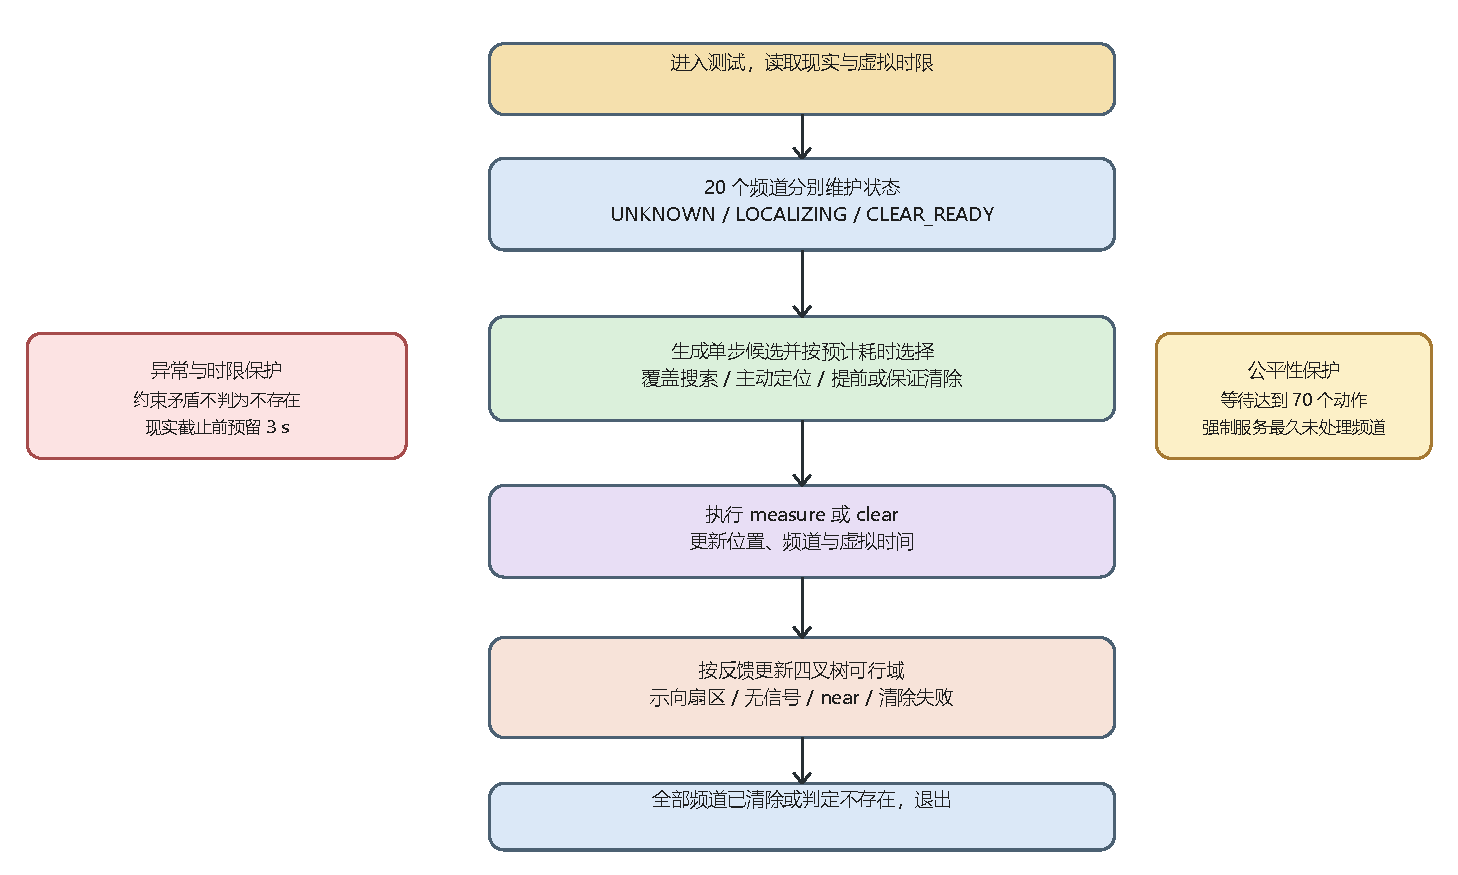
\includegraphics[width=0.88\textwidth]{figures/q3_consistent/flow.pdf}
  \caption{与实际程序一致的多频道搜索、定位与清除流程}
  \label{fig:q3-flow}
\end{figure}

\subsection{参数设置与离线实验}

\subsubsection{当前运行参数}

正式入口优先读取随提交程序提供的当前参数文件；仅当该文件不存在时，才退回程序类中定义的缺省值。因此，表~\ref{tab:q3-params} 列出的是本次运行实际加载的当前参数，而不是缺省参数。当前算法模块的 SHA-256 摘要前 16 位为 \texttt{69a36076e32dfa8e}，与运行日志记录的 16 位算法版本标识一致。

\begin{table}[htbp]
  \centering
  \caption{问题三程序当前参数}
  \label{tab:q3-params}
  \begin{tabular}{llll}
    \toprule
    参数 & 数值 & 参数 & 数值\\
    \midrule
    四叉树停止边长上限 & $14\,\mathrm m$ & 搜索环半径 & $1450\,\mathrm m$\\
    定位代表点数 & 21 & 清除候选代表点数 & 15\\
    横向偏移 & $40,100,220\,\mathrm m$ & 提前清除阈值 & 0.55\\
    最大主动定位次数 & 6 & 最大失败清除次数 & 2\\
    最大延后动作数 & 70 & 现实时间余量 & $3\,\mathrm s$\\
    目标不确定度尺度 & $12\,\mathrm m$ & 交会正弦下限 & 0.015\\
    \bottomrule
  \end{tabular}
\end{table}

程序另提供离线参数迭代流程：同一批案例比较当前参数与候选参数，每第五个案例作为验证案例；训练优胜者必须全部清除，验证集也必须全部清除，且在当前参数无失败时，验证目标 $0.8\bar T+0.2T_{90}$ 不得劣化超过 $2\%$。该流程用于选择效率参数，不改变题目物理常量与误差安全边界。

\subsubsection{实验设计与总体结果}

为核对论文和程序的一致性，本文直接调用附件中的离线环境，对当前参数独立运行 36 局，种子依次为 104027--104062。空间分布包含圆域内按面积均匀、半径 $1800\,\mathrm m$ 的边界分布，以及方位集中在 $\pm0.2$ 弧度且半径为 $700$--$1100\,\mathrm m$ 的聚集分布；误差模式包含空间固定误差场、固定 $+1^\circ$ 和固定 $-1^\circ$。九种“空间分布--误差模式”组合各出现 4 次，目标个数由程序在 $10$--$16$ 中随机生成。算法运行时不可读取真值，真值只用于局后评价。

36 局均清除全部干扰源。表~\ref{tab:q3-overall-results} 给出总体统计。这里的平均定位清除时间按题目口径，对每局的“虚拟总时间/实际清除数”再取平均；P90、P95 和最慢 $20\%$ 均按 36 个虚拟总时间计算。

\begin{table}[htbp]
  \centering
  \caption{当前程序 36 局离线评测总体结果}
  \label{tab:q3-overall-results}
  \resizebox{\textwidth}{!}{%
  \begin{tabular}{lrrrrrrrr}
    \toprule
    完成率 & 平均总时间/s & P90/s & P95/s & 最慢20\%平均/s & 平均定位清除时间/s & 平均动作数 & 平均移动距离/m & 平均失败清除数\\
    \midrule
    36/36 & 5431.7 & 7477.0 & 8187.5 & 7651.4 & 424.4 & 114.9 & 23874 & 4.1\\
    \bottomrule
  \end{tabular}}
\end{table}

\begin{figure}[htbp]
  \centering
  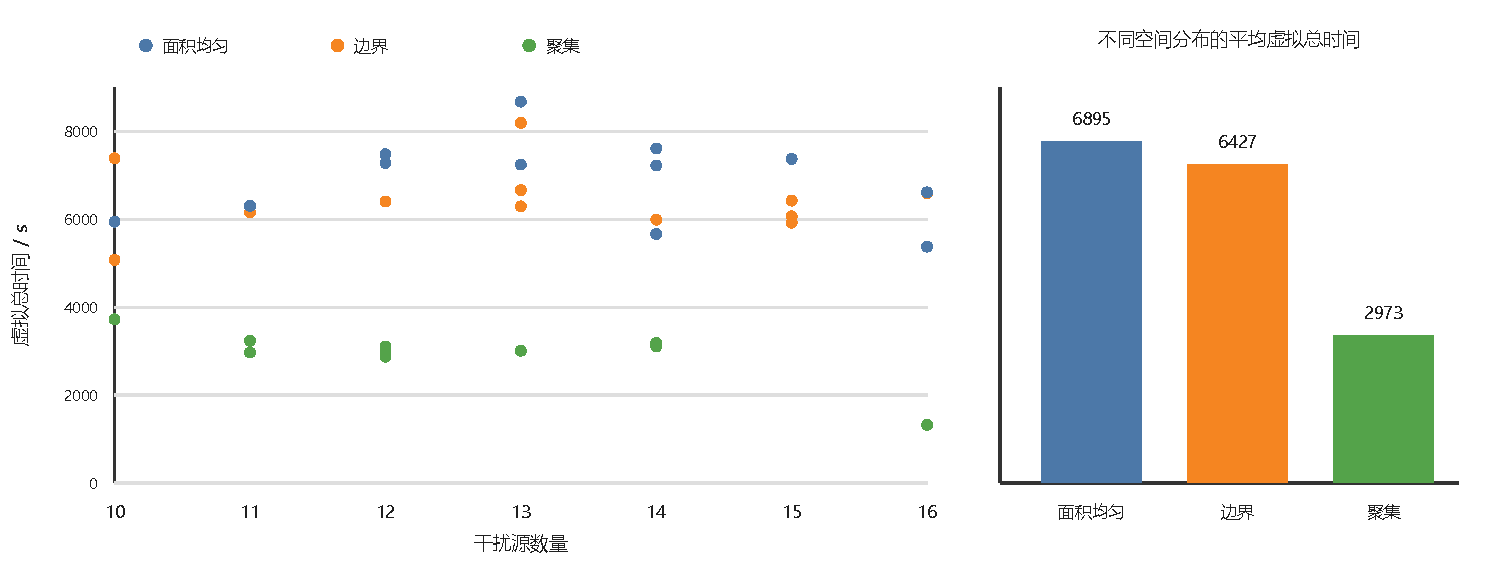
\includegraphics[width=0.98\textwidth]{figures/q3_consistent/results.pdf}
  \caption{36 局虚拟总时间散点与不同空间分布的均值}
  \label{fig:q3-results}
\end{figure}

从图~\ref{fig:q3-results} 可见，聚集场景平均耗时为 $2973\,\mathrm s$，低于面积均匀场景的 $6895\,\mathrm s$ 和边界场景的 $6427\,\mathrm s$。这是因为聚集目标更容易在相近位置连续定位和清除；均匀及边界分布则需要更长移动路线。目标数并非唯一决定因素：目标较少时，算法仍需通过更多无信号检测排除空频道，而目标较多时又会增加定位与清除任务，两种效应共同决定总时间。

\subsubsection{候选参数敏感性}

程序附带四组待验证候选，分别单独改变目标不确定度尺度、最大延后动作数、四叉树停止边长上限和定位代表点数。为避免不同案例造成偏差，本文让当前参数与四组候选在上述同一批 36 个场景上运行，共得到 180 局记录。表~\ref{tab:q3-candidates} 中的综合目标按程序定义计算为 $0.8\bar T+0.2T_{90}$。

\begin{table}[htbp]
  \centering
  \caption{当前参数与四组单参数候选的同场景比较}
  \label{tab:q3-candidates}
  \begin{tabular}{lrrrr}
    \toprule
    配置（相对当前参数的变化） & 完成率 & 平均总时间/s & P90/s & 综合目标/s\\
    \midrule
    定位代表点 $21\to15$ & 36/36 & 5427.3 & 7460.6 & 5834.0\\
    当前参数 & 36/36 & 5431.7 & 7477.0 & 5840.8\\
    不确定度尺度 $12\to8\,\mathrm m$ & 36/36 & 5457.2 & 7384.2 & 5842.6\\
    叶格上限 $14\to28.2\,\mathrm m$ & 36/36 & 5516.6 & 7534.8 & 5920.2\\
    最大延后动作 $70\to50$ & 36/36 & 7171.6 & 10022.7 & 7741.8\\
    \bottomrule
  \end{tabular}
\end{table}

五组参数均完成全部场景，说明这些效率参数未破坏硬约束闭环。将定位代表点数由 21 减至 15 的平均总时间仅下降 $4.4\,\mathrm s$，约为 $0.08\%$，差异很小；过早把最大等待阈值降至 50 则显著增加往返，总时间上升约 $32.0\%$。因此，当前结果能够明确否定“更频繁强制公平调度一定更快”，但不足以证明代表点数 15 在官方环境中稳定优于 21。为遵守程序与论文的一致性，正文总体结果仍以附件实际加载的当前参数为准，不在论文阶段替换参数文件。

按目标个数统计的结果见表~\ref{tab:q3-by-count}。由于各组只有 4--7 局，表中均值用于说明程序行为，不据此作单调性结论。

\begin{table}[htbp]
  \centering
  \caption{当前程序按干扰源个数分组的离线表现}
  \label{tab:q3-by-count}
  \begin{tabular}{rrrrrr}
    \toprule
    目标数 & 场景数 & 平均总时间/s & 平均定位清除时间/s & 平均动作数 & 平均移动距离/m\\
    \midrule
    10 & 4 & 5529.3 & 552.9 & 128.3 & 23965\\
    11 & 4 & 4662.3 & 423.8 & 112.8 & 20074\\
    12 & 7 & 4733.2 & 394.4 & 111.4 & 20482\\
    13 & 6 & 6675.7 & 513.5 & 119.8 & 29928\\
    14 & 7 & 5131.2 & 366.5 & 106.7 & 22629\\
    15 & 4 & 6443.3 & 429.6 & 126.5 & 28576\\
    16 & 4 & 4974.4 & 310.9 & 105.0 & 21915\\
    \midrule
    合计 & 36 & -- & -- & -- & --\\
    \bottomrule
  \end{tabular}
\end{table}

\subsubsection{典型场景分析}

选取种子 104046 的边界分布、空间误差场场景。该局含 13 个干扰源，全部清除，共用时 $6659.2\,\mathrm s$，执行 136 个动作；移动距离为 $29400.8\,\mathrm m$，检测 117 次、切换频道 111 次、清除 19 次，其中失败 6 次。平均定位清除时间为 $512.2\,\mathrm s$。图~\ref{fig:q3-trajectory} 中的真值只在运行结束后用于画图，未提供给算法。

\begin{figure}[H]
  \centering
  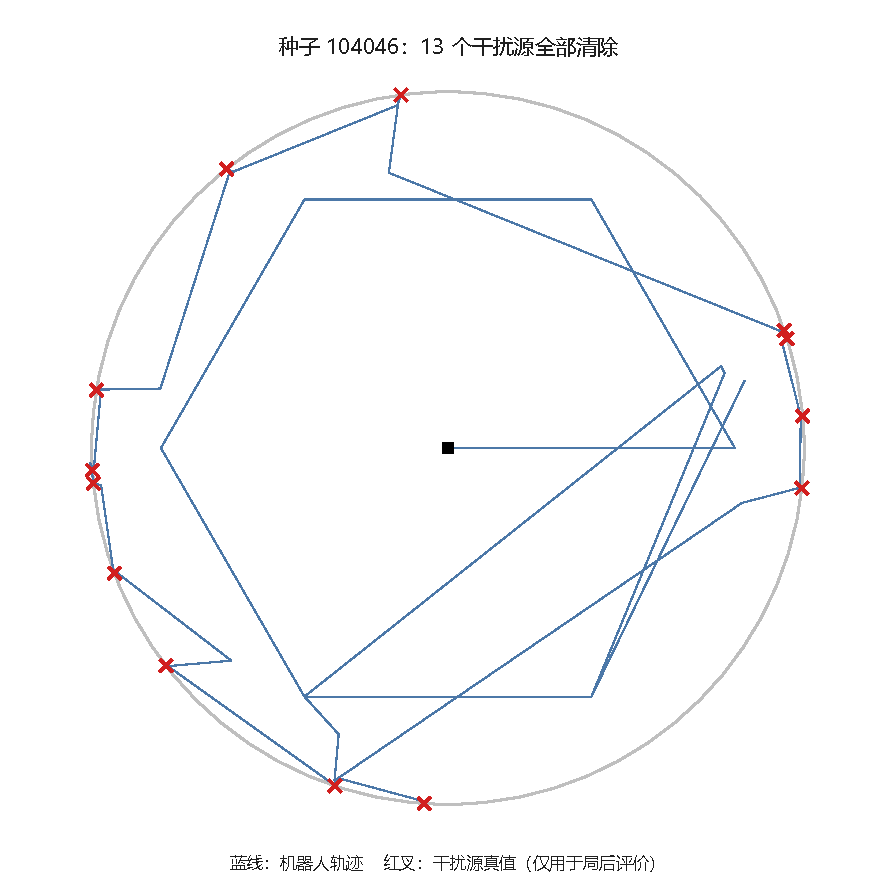
\includegraphics[width=0.56\textwidth]{figures/q3_consistent/trajectory.pdf}
  \caption{种子 104046 场景的机器人轨迹与干扰源真值}
  \label{fig:q3-trajectory}
\end{figure}

该局移动耗时为 $5880.2\,\mathrm s$，占总时间约 $88.3\%$；检测耗时 $585\,\mathrm s$，频道切换耗时 $111\,\mathrm s$，成功与失败清除分别耗时 $65\,\mathrm s$ 和 $18\,\mathrm s$。图~\ref{fig:q3-time-breakdown} 表明，减少长距离往返仍是后续优化的首要方向。

\begin{figure}[H]
  \centering
  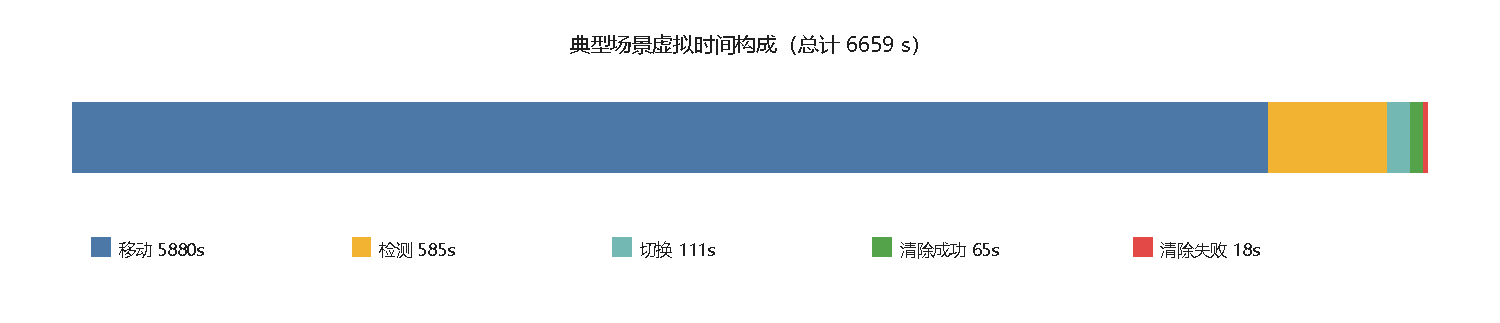
\includegraphics[width=0.88\textwidth]{figures/q3_consistent/time_breakdown.pdf}
  \caption{典型场景的虚拟时间构成}
  \label{fig:q3-time-breakdown}
\end{figure}

\subsection{模型评价与适用边界}

本策略的主要优点是：七点骨架给出确定的频道发现条件；四叉树裁剪始终保留边界不确定性；\texttt{near}、保证清除和有限覆盖兜底使已发现频道具有明确的清除路径；公平性和时限保护避免频道长期搁置或临界超时。当前 36 局离线实验全部完成，说明程序在所设三类空间分布和三类误差模式下能够闭环运行。

需要强调，代表点比例、误差传播式和惩罚项均是效率启发式，不是目标位置概率模型；离线环境的误差场也不能替代官方模拟器。表~\ref{tab:q3-overall-results} 中的 36/36 仅表示上述离线环境下 36 个可复现场景全部完成，不能解释为正式测试的清除率。附件中未包含其说明文档所提到的独立单元测试文件，因此本文不再保留旧稿“38 项单元测试全部通过”的结论。现有数值只对应当前程序、当前参数及上述离线场景，不与未包含在程序中的基线、联合停靠或双目标共享版本作比较。正式提交前仍应在官方模拟器上记录完成率和实际耗时，并据此决定是否继续调整效率参数。
